 %------------------第四章---------------------------
    \newpage
	\section{传感器程序设计}
    \subsection{传感器检测原理与检测策略}
    

    
    \subsubsection{检测原理}
    超声波一般指振动频率超过20KHz的脉冲波,其具有频率高、波长锻、穿透性强以及绕射性小等特点\upcite{检测原理},当遇到杂质或材料分界面时,会产生显著的反射效应形成回波利用回波信号可进行距离检测、表面缺陷排查、材质判断等方面的应用,而本设计中超声波传感器则用于生产线钢化玻璃的接近检测。
    超声波信号的振幅会随其传播距离的增大而不断减小,通过滤波解调等处理,可将回波信号处理成一个简单的单峰信号,如公式\ref{VOUT公式}以及图\ref{回波接收模块}所示,将不同距离的回波进行处理,可以得到不同峰值的单峰信号,通过检测峰值来判断物体是否到达指定位置。
    如图\ref{VOUT输出},为20V驱动电压下, LNA\_GAIN = 0x0; VOUT\_SCALE\_SEL = 0x0; 
LOGAMP\_DIS\_FIRST = 0x0; LOGAMP\_DIS\_LAST = 0x0时不同距离对应VOUT的输出,可以看到,随着检测距离的减小,VOUT输出的峰值也在不断减小。\par
    \begin{figure}[H]
        \centering
        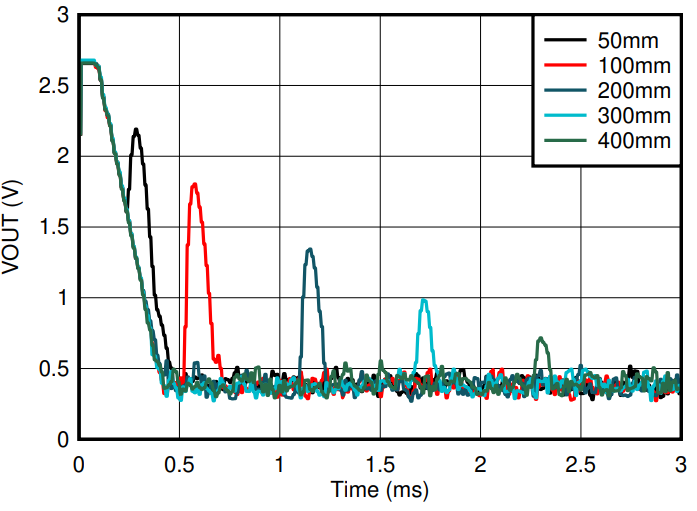
\includegraphics[width=10cm]{figure/VOUT image.png}
        \caption{VOUT输出}
        \label{VOUT输出}
    \end{figure}
    在应用中,首先通过SPI接口向ECHO\_INT\_CONFIG寄存器配置VOUT引脚的阈值,当引脚的电压超过所配置的阈值时,即判断为检测到了物体,OUT4引脚拉高,将其作为控制信号连接至MCU。\par
    TUSS4470驱动芯片还提供了过零检测的功能,通过OUT3引脚输出的过零信号,可对回波频率进行再次检测,增加对其它信号的抗干扰性。该过零信号来自图\ref{TUSS4470芯片功能框图}
    中的对数模块,当信号在其中进行解调时,可根据应用选取特定阶段的信号作为零点。该过零信号仅在OUT4拉高时才有输出,以避免其它噪声的干扰。
    \subsubsection{检测策略}
      在配置完成TUSS4470驱动芯片后,即可开始产生脉冲信号并通过超声换能器发送脉冲波。与传统的超声波传感器不同,采用该驱动芯片可发送指定次数、指定脉冲数的脉冲波,这就为我们设计丰富的检测策略提供了硬件基础。考虑到钢化玻璃处于复杂的工厂环境,传感器易受到各种电磁信号的影响,因此增加传感器的稳定性就变得至关重要。\par
      本设计采用多次发射脉冲波的检测策略,在发送完一次指定脉冲数的脉冲波之后,传感器就进入检测模式,假如检测到了有效回波,检测标志位加一。连续发射五次脉冲,以五次脉冲波的发射作为一次检测周期,每个检测周期后都会更新检测状态。当一个检测周期内有超过三次检测到有效回波时,判断为检测到物体,DETECTED\_STATE=1,LED灯亮;有效脉冲波的次数小于或等于三次时,判断为未检测到物体,DETECTED\_STATE=0,\par\noindent LED灯灭。如图\ref{检测逻辑流程图}为实现检测逻辑的程序流程图,图\ref{检测状态转移图}为检测状态转移图。
     \begin{figure}[H]
      \begin{minipage}{0.5\linewidth}
		\centering
		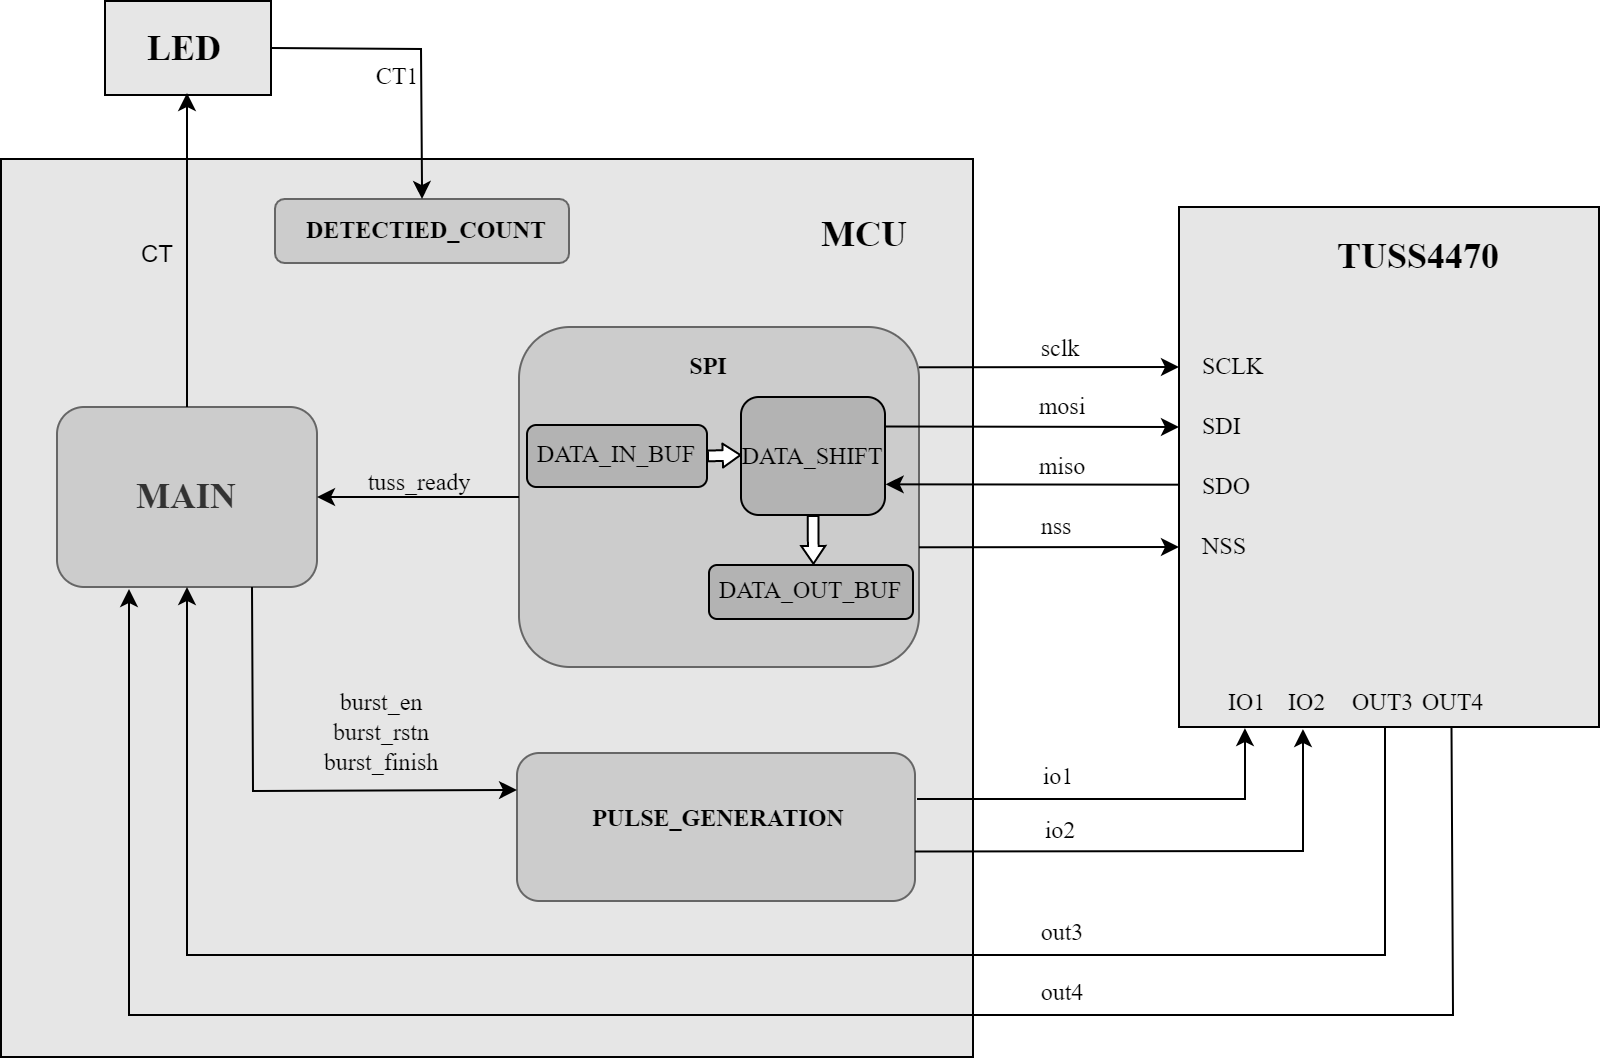
\includegraphics[width=5cm]{figure/Overall program block diagram.png}
		\caption{检测逻辑流程图}
		\label{检测逻辑流程图}%文中引用该图片代号
	\end{minipage}
	%\qquad
	\begin{minipage}{0.4\linewidth}
		\centering
		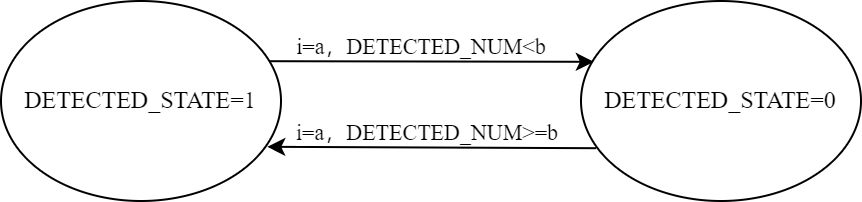
\includegraphics[width=5cm]{figure/LED state transition diagram.png}
		\caption{检测状态转移图}
		\label{检测状态转移图}%文中引用该图片代号
	\end{minipage}
\end{figure}
    此种检测策略可以极大的增加传感器的稳定性,只有在指定位置持续检测到钢化玻璃时才会认为检测到物体,一定程度上可以避免发生因外界干扰而出现错误检测的情况。
    
      
      
  
      
    
    \subsection{传感器程序设计,解释代码}
    \subsubsection{程序总体设计}
    本设计所使用的EPM240T100C5N芯片采用Verilog HDL作为编程语言,Quartus II作为编程烧录软件。Verilog HDL\upcite{Verilog介绍}是一种硬件描述语言(HDL:Hardware Description Language),以文本形式来描述数字系统硬件的结构和行为的语言,用它可以表示逻辑电路图、逻辑表达式,还可以表示数字逻辑系统所完成的逻辑功能。\par
    在本设计中,如图\ref{程序整体框图}所示,将MCU分成四个模块,分别是:MAIN模块、SPI模块、PULSE\_GENERATION模块、DETECTED\_COUNT模块,实现配置TUSS4470芯片、产生脉冲信号、到位指示以及计数等功能。
    
         \begin{figure}[H]
        \centering
        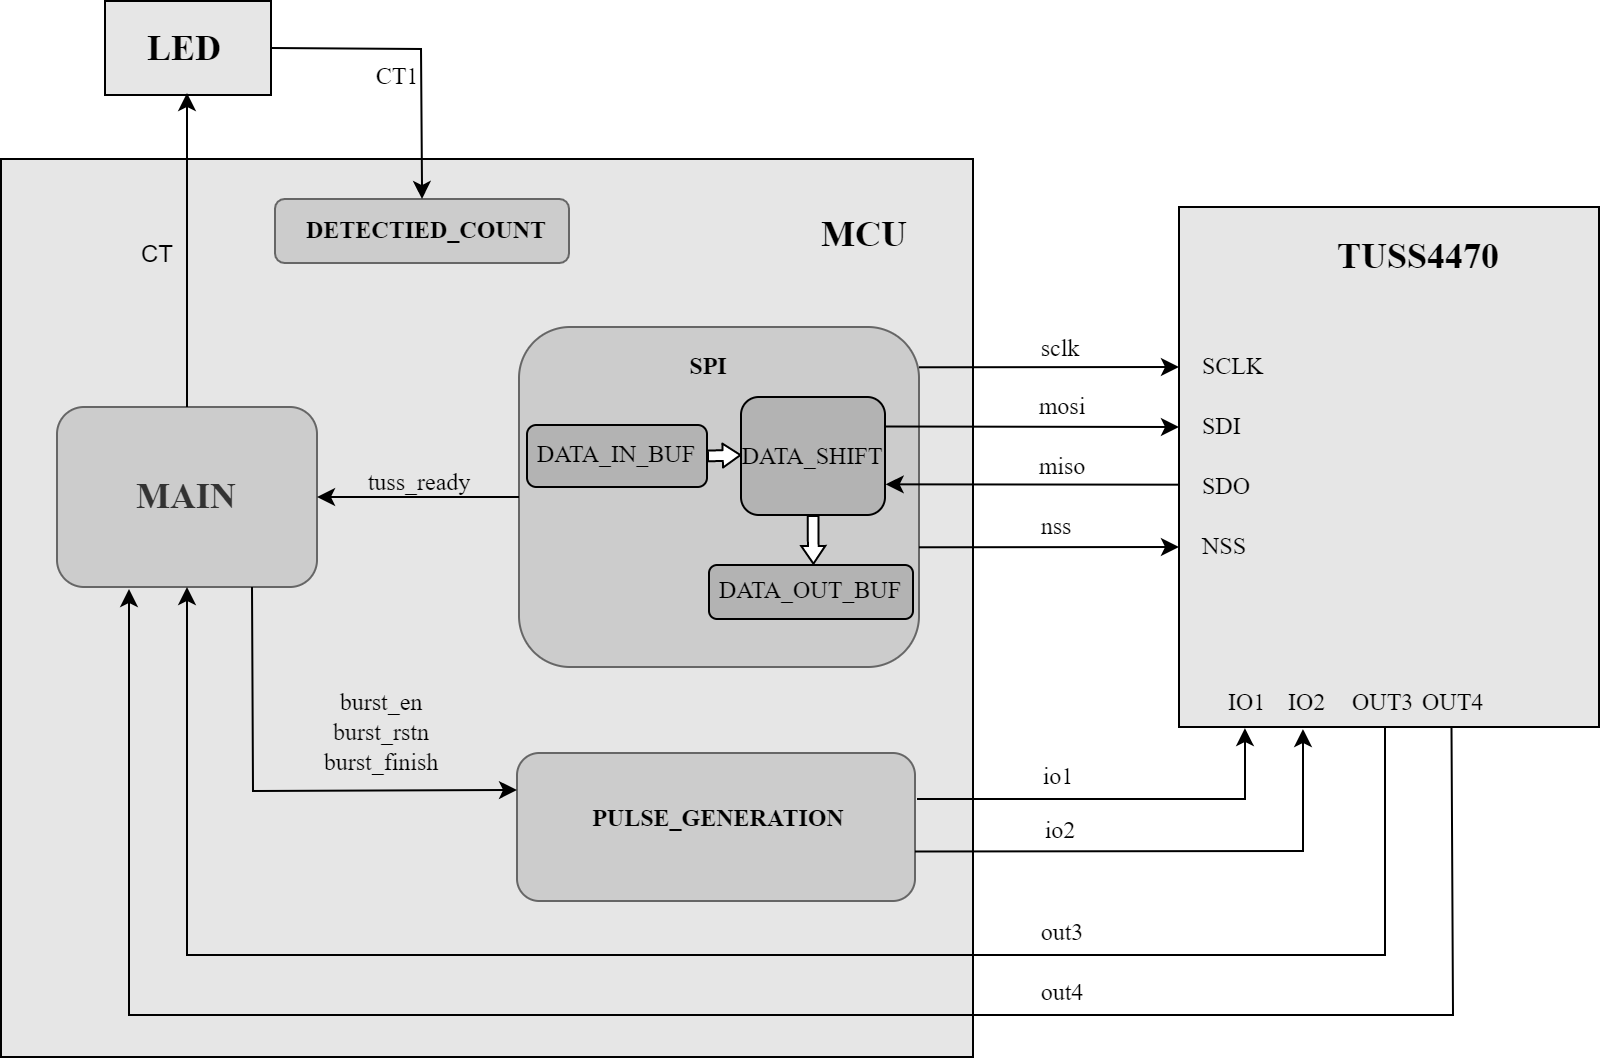
\includegraphics[width=12cm]{figure/Overall program block diagram.png}
        \songti\zihao{5}\caption{程序整体框图}
        \label{程序整体框图}
    \end{figure}
    
    \subsubsection{控制模块}
    图\ref{程序整体框图}中的MAIN模块为传感器的控制模块,其作用在于,协调各模块间的工作,是程序的主要部分,图\ref{MAIN模块程序流程图}为MAIN模块的工作流程图。
    首先是SPI模块向TUSS4470芯片发送配置数据,并接收从TUSS4470反馈回的芯片状态;根据反馈数据判断芯片是否准备就绪,当准备就绪后向MAIN模块发送tuss\_ready信号;之后通过IO1、IO2引脚配合控制产生脉冲信号,在每次发送完脉冲信号后,都会根据OUT3、OUT4引脚返回的信息判断本次是否检测到物体;多次检测到预定回波后即确认为检测到物体,通过CT引脚控制LED灯亮;检测计数模块也将进行计数。
    \begin{figure}[H]
        \centering
        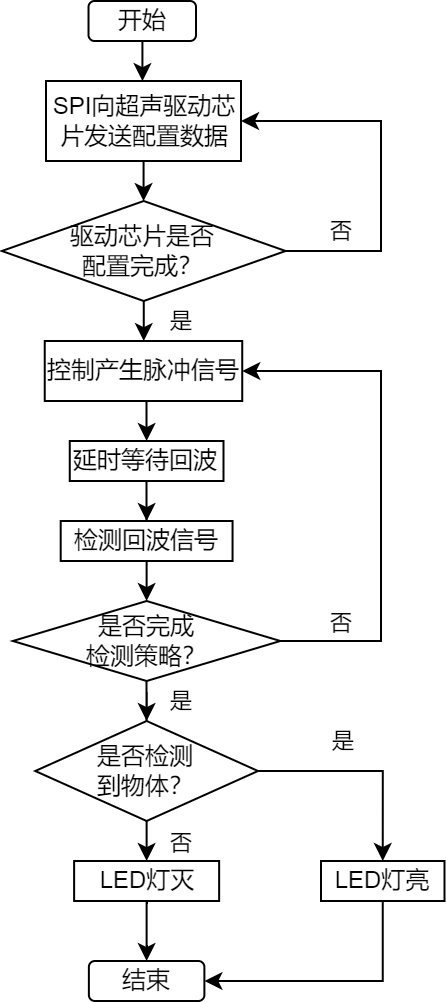
\includegraphics[width=5cm]{figure/MAIN module flow chart.png}
        \songti\zihao{5}\caption{MAIN模块程序流程图}
        \label{MAIN模块程序流程图}
    \end{figure}
    
    
    
    \subsubsection{SPI通信模块}
    \noindent
    \textbf{1、介绍}\par
    在本设计中,MCU芯片通过SPI通信协议来配置TUSS4470芯片。SPI\upcite{SPI}是串行外设接口(Serial Peripheral Interface)的缩写,是Motorola公司推出的一种同步串行接口技术,是一种高速、全双工、同步的通信总线。\par
    在本设计中,采用的是四线制SPI,其包括:SCLK(时钟信号)、NCS(片选信号)、MOSI(MCU输出信号)、MISO(MCU输入信号)。SCLK时钟信号和NCS片选信号都由主设备产生,NCS信号拉低为有效信号。
    
    \noindent
    \textbf{2、模式选择}\par
    SPI通信模式通过CPOL(时钟极性)和CPHA(时钟相位)来确定。其中CPOL配置SCLK电平的有效态,当CPOL=0时,SCLK低电平处于空闲态,高电平有效,当CPOL=1时,SCLK高电平为空闲态,低电平有效;CPHA配置数据采样发生在第几个边沿,当CPHA=0时,在第一个边沿数据采样,在第二个边沿数据发送,当CPHA=1时,在第一个边沿数据发送,在第二个边沿数据采样。\par
    根据芯片手册可以得知驱动芯片为高电平有效,在上升沿接收数据,在下降沿发送数据,即MCU在上升沿发送数据,在下降沿接收数据,可以得知选择的SPI模式为:CPOL=0,CPHA=1。
    
    \noindent
    \textbf{3、实现原理}\par
    SPI的全双工通信通过一个移位寄存器DATA\_SHIFT来实现。待发送的数据首先写入DATA\_IN\_BUF中进行缓存,需要发送时写入DATA\_SHIFT中,通过移位先将高位数据发送给从机,再将接收到的数据存储到低位,以8位的移位寄存器为例,其工作示意图如图\ref{移位寄存器工作示意图}所示,当发送完成8位数据11110000时,也完成了数据的接收。在接收完成数据后,将数据存入到DATA\_OUT\_BUF寄存器中,至此实现了一帧数据的收发流程。
        \begin{figure}[H]
        \centering
        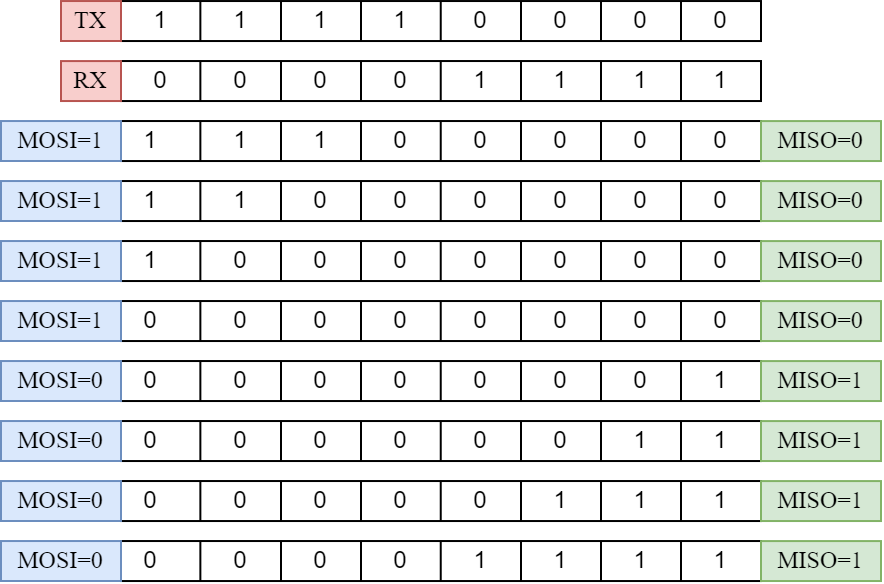
\includegraphics[width=10cm]{figure/DATA_SHIFT.png}
        \songti\zihao{5}\caption{移位寄存器工作示意图}
        \label{移位寄存器工作示意图}
    \end{figure}
    
    
    \noindent
    \textbf{4、程序设计}\par
    单帧数据的发送采用线性序列机的方式来实现,即利用一个计数器不断计数,计数器的每一个值都对应一个时刻,在不同时刻对DATA\_SHIFT寄存器采取不同操作,如表\ref{线性序列机}所示。当复位时,对DATA\_SHIFT寄存器进行初始化;当计数器CNT为0时,将DATA\_IN\_BUF内的数据赋值给DATA\_SHIFT;当CNT为1-16时,DATA\_SHIFT寄存器进行移位操作;当CNT=17时,将DATA\_SHIFT内的数据赋值给DATA\_OUT\_BUF,至此单帧数据收发完毕,在这基础上,将进行多帧数据的收发。
    
    \begin{table}[H]
        \centering
        \caption{线性序列机}
    \begin{tabular}{c|c}
    \hline
    CNT & 操作  \\ \hline
    复位 & \begin{lstlisting}
        DATA_SHIFT=0;DATA_OUT_BUF=0;
            \end{lstlisting}    \\ \hline
    
    0 & \begin{lstlisting}
        DATA_SHIFT=DATA_IN_BUF;
        \end{lstlisting}   \\ \hline
    
    1-16&  \begin{lstlisting}
    mosi<=DATA_SHIFT[15];DATA_SHIFT<={DATA_SHIFT[14:0],miso};
            \end{lstlisting} \\ \hline
    
    17&     \begin{lstlisting}
        DATA_OUT_BUF<=DATA_SHIFT;
            \end{lstlisting}  \\ \hline
            
        \end{tabular}
                \label{线性序列机}
    \end{table}
    
    TUSS4470芯片采用高位先发的方式来收发数据,当NCS信号拉低时,SPI模块开始工作,当NCS拉高,SPI模块停止工作,完成一帧数据的收发。SPI无法实现连续收发多帧的数据,在每帧数据的收发之间NCS需要经历低-高-低的过程。实现多帧数据收发的程序流程图如图\ref{收发多帧数据程序流程图}所示,该程序可一次性发送9帧16位的数据至TUSS4470驱动芯片。
    \begin{figure}[H]
        \centering
        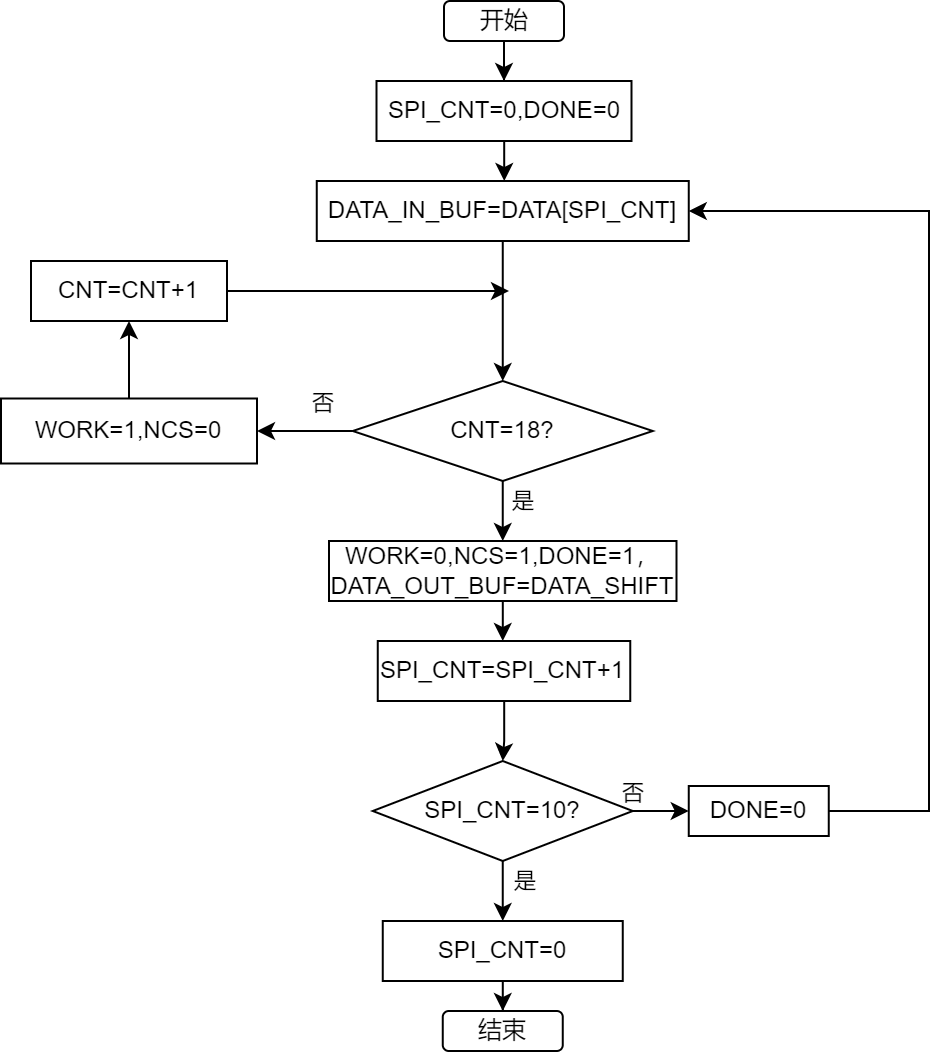
\includegraphics[width=10cm]{figure/SPI Program Flow Chart.png}
        \songti\zihao{5}\caption{收发多帧数据程序流程图}
        \label{收发多帧数据程序流程图}
    \end{figure} 
    图中SPI\_CNT用于记录收发数据的帧数;DONE为每帧数据发送完成标志位;WORK为工作位,用于记录工作状态;DATA为一个$10\times16$的数组,用于存放配置数据。
    程序开始运行后,首先进行数据初始化,然后将DATA寄存器内的数据赋给DATA\_IN\_BUF寄存器,片选信号NCS拉低,进行单帧数据的收发。当CNT=18时完成单帧数据的收发,DONE置1,片选信号NCS拉高,帧数计数位SPI\_CNT+1,DONE、CNT置零。在将DATA内的数据发送完成后,根据驱动芯片返回的数据判断芯片是否完成配置,如果完成配置,SPI通信模块将向main模块发送tuss\_ready信号,反之则重新进行配置。
    
    
    

    
    \noindent
    \textbf{5、数据结构}\par
    图\ref{SPI数据结构图1}为SPI通信的数据结构图
    \begin{figure}[H]
        \centering
        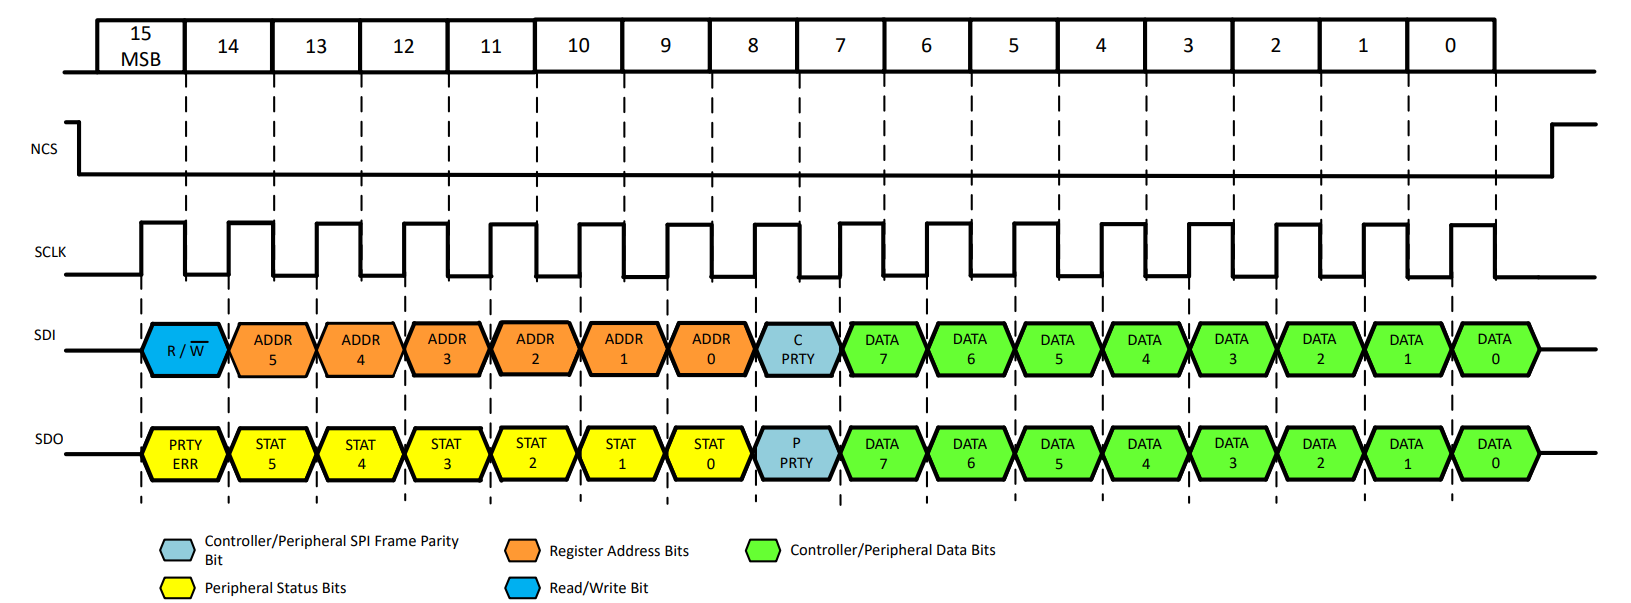
\includegraphics[width=10cm]{figure/SPI Frame.png}
        \songti\zihao{5}\caption{SPI数据结构图1}
        \label{SPI数据结构图1}
    \end{figure}
    MCU通过SDI引脚向驱动芯片发送配置数据,通过SDO引脚接收驱动芯片返回的数据。SDI发送数据的第15位为读写选择位,当其选择为write模式或者read模式时,数据收发数据的结构都有所不同,如图\ref{SPI数据结构图2}所示。
    \begin{figure}[H]
        \centering
        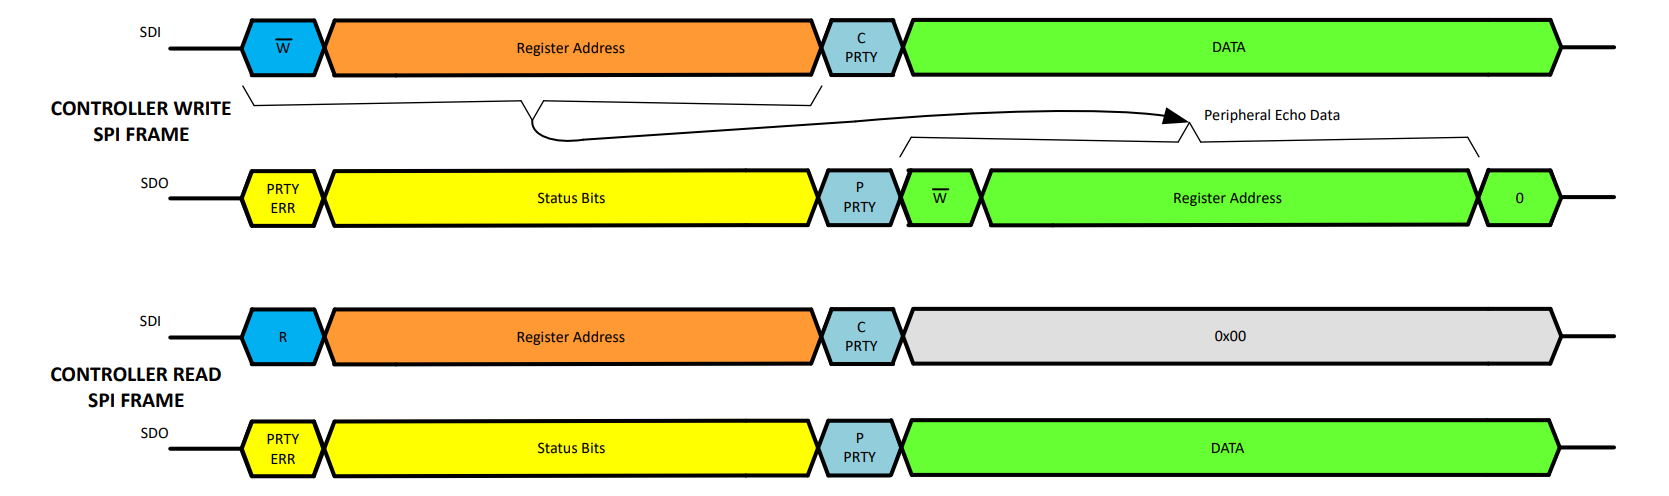
\includegraphics[width=12cm]{figure/SPI Transfer Sequence.png}
        \songti\zihao{5}\caption{SPI数据结构图2}
        \label{SPI数据结构图2}
    \end{figure}
    在write模式下,SDI14位-9位为寄存器地址,第8位为奇校验位,7位-0位为寄存器配置数据。SDO第一位为奇校验错误位,用于记录发送数据的奇校验是否通过,未通过校验时该位置1,14位-9位为驱动芯片的状态位,用于反映芯片当前的状态模式,如表\ref{芯片状态表}所示。第8位为奇校验位,7位-0位为写入寄存器的地址。\par
    
    \begin{table}[H]
        \centering
        \zihao{5}\caption{芯片状态表}
        \songti\zihao{5}
        \begin{tabular}{c|c}
            \hline
            \textbf{STATUS BIT }& \textbf{DESCRIPTION}      \\ \hline
            STAT 5 - VDRV\_READY    &   VDRV引脚达到配置电压值时置1  \\ \hline
            STAT 4 - PULSE\_NUM\_FLT &  发生脉冲数目错误是置1  \\\hline
            STAT 3 - DRV\_PULSE\_FLT &  脉冲发生无响应时置1 \\\hline
            STAT 2 - EE\_CRC\_FLT & 加载内部EEPROM存储器出现CRC错误时置1\\\hline
            STAT <1:0> - DEV\_STATE  &  \makecell{芯片模式:\\
                                        00 - 检测模式\\
                                        01 - 脉冲发生模式\\
                                        10 - 待机模式\\
                                        11 - 睡眠模式} \\\hline
            
      
            \end{tabular}
        \label{芯片状态表}    
         \end{table}
    在read模式下,SDI的14位-9位为读取寄存器地址,7位-0位为0,SDO的7位-0位为该寄存器内存储的数据。
    
    


    
    \noindent
    \textbf{6、寄存器配置}\par
    TUSS4470超声驱动芯片各寄存器的配置如表\ref{寄存器配置}所示。
      \begin{table}[H]
        \centering
        \zihao{5}\caption{寄存器配置}
        \songti\zihao{5}
        \begin{tabular}{c|c|c|c}
        \hline
        \textbf{寄存器名} & \textbf{缩写}& \textbf{地址} &\textbf{配置值}\\ \hline
        Bandpass filter settings&BPF\_CONFIG\_1&0x10& 0x25 \\ \hline
        Bandpass filter settings&BPF\_CONFIG\_2&0x11& 0x00\\ \hline
        Log-amp configuration&DEV\_CTRL\_1&0x12& 0xB3\\ \hline
        Log-amp configuration&DEV\_CTRL\_2&0x13& 0x02\\ \hline
        Log-amp configuration&DEV\_CTRL\_3&0x14& 0x03\\ \hline
        VDRV Regulator Control&VDRV\_CTRL&0x16& 0x07\\ \hline
        Echo Interrupt Control &ECHO\_INT\_CONFIG&0x17&0x0F \\ \hline  
        Zero Crossing configuration &ZC\_CONFIG&0x18& 0xD4\\ \hline 
        Burst pulse configuration &BURST\_PULSE&0x1A& 0x08\\ \hline 
        Time of Flight Config&TOF\_CONFIG&0x1B& 0x00\\ \hline 
        Fault status bits&DEV\_STAT&0x1C& 0x00\\ \hline
        Device ID&DEVICE\_ID&0x1D& 0x00\\ \hline
        Revision ID &REV\_ID&0x1E& 0x00\\ \hline
        
            \end{tabular}
        \label{寄存器配置}    
         \end{table}
    其中BPF\_CONFIG\_1用于配置带通滤波器的中心频率,该频率需匹配超声波传感器的工作频率,查阅芯片手册可以得知,当寄存器配置为0x25时,带通滤波器的中心频率为301.28KHZ,与超声波传感器最匹配;\par
    BPF\_CONFIG\_2用于设置滤波器的Q因素,修正滤波器的频率范围;\par
    DEV\_CTRL\_1用于调整对数放大器参数,通过查阅资料,将其设置为0xB3;\par
    DEV\_CTRL\_2用于设置放大器(LNA)的增益;\par
    DEV\_CTRL\_3用于配置脉冲发生的模式,本设计采用IO\_MODE3,故将该寄存器配置为0x03;\par
    VDRV\_CTRL寄存器主要用于配置VDRV引脚的参考电压,当该引脚的实际电压超过参考电压时,驱动芯片的VDRV\_READY状态位置1,然后通过SPI将该状态位返回至MCU芯片。本设计采用12V的驱动电压,根据芯片手册所给出的公式得出该寄存器配置为0x0F;\par
    ECHO\_INT\_CONFIG用于配置VOUT引脚的参考阈值,当VOUT引脚输出电压超过该阈值时,即判断为检测到物体,OUT4拉高。本设计所需的检测距离为200mm,根据实验将电压阈值设置为1V,寄存器配置为0x0F;\par
    ZC\_CONFIG寄存器用于配置过零信号,以提高传感器的抗干扰性。选取380mV作为零点,配合OUT4信号进行接近检测,寄存器配置为0xD4;\par
    BURST\_PULSE寄存器的前五位用于配置每个脉冲波的脉冲数,本设计的脉冲数为8,故配置其为0x08;\par
    TOF\_CONFIG寄存器用于待机模式和睡眠模式的设置,本设计只使用到脉冲发生模式和检测模式,暂不需要使用到这两种模式,故配置为0x00;\par
    DEV\_STAT寄存器为芯片的状态寄存器,包括了VDRV状态、脉冲发生状态,可供MCU芯片读取,故不需写入数据,配置为0x00;\par
    DEVICE\_ID和REV\_ID寄存器存放的是芯片的固定参数,无需写入,配置为0x00。
    
    \subsubsection{脉冲发生模块}
    TUSS4470超声驱动芯片有4种脉冲模式来为超声传感器提供激励。在每个模式中,超声发出脉冲的频率取决于外部输入时钟的频率,这可以让使用者产生精确的时钟来匹配超声波传感器的固有频率,从而产生最高的声压水平。在本设计中,将采用脉冲模式1来产生脉冲信号。\par
    在脉冲模式1中,IO2引脚将作为外部时钟输入引脚,IO1作为控制引脚。如图\ref{脉冲模式1}所示,当IO1引脚拉低时,进入脉冲发生模式,在检测到IO2引脚的第一个下降沿时,开始产生脉冲,产生脉冲的数目将通过下降沿的个数来计算。4当产生脉冲的数目达到寄存器内的配置值,或者IO1引脚的信号拉高时,都将退出脉冲发生模式,取决于哪个事件先发生。在进入到脉冲发生模式后,OUTA和OUTB引脚的信号都将取决于IO1和IO2引脚,当需要连续产生多次脉冲时,IO2引脚的信号需要经历低-高-低的过程。
     \begin{figure}[H]
        \centering
        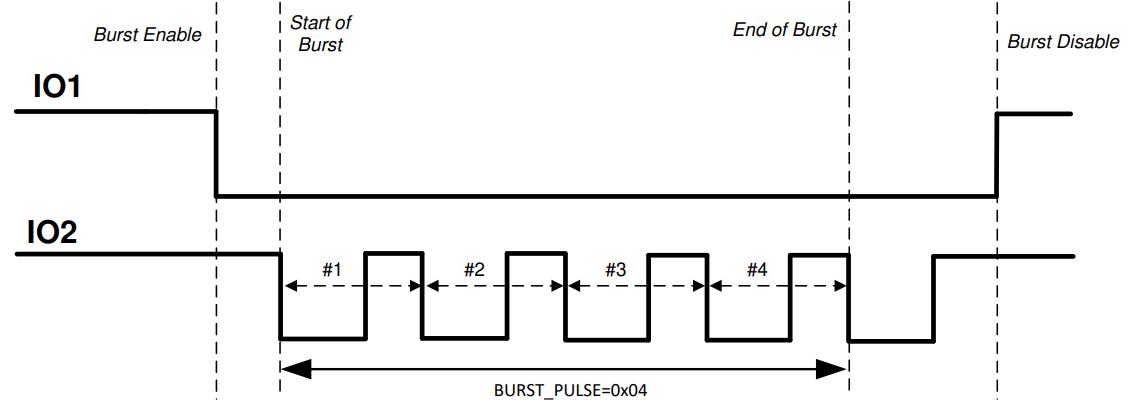
\includegraphics[width=12cm]{figure/IO MODE1.png}
        \songti\zihao{5}\caption{脉冲模式1}
        \label{脉冲模式1}
    \end{figure}
    在本设计的脉冲发生模块中,将能产生指定频率,指定脉冲数,指定次数的脉冲波,程序流程图如图所示。
    
   
    
    
    
       \begin{figure}[H]
        \centering
        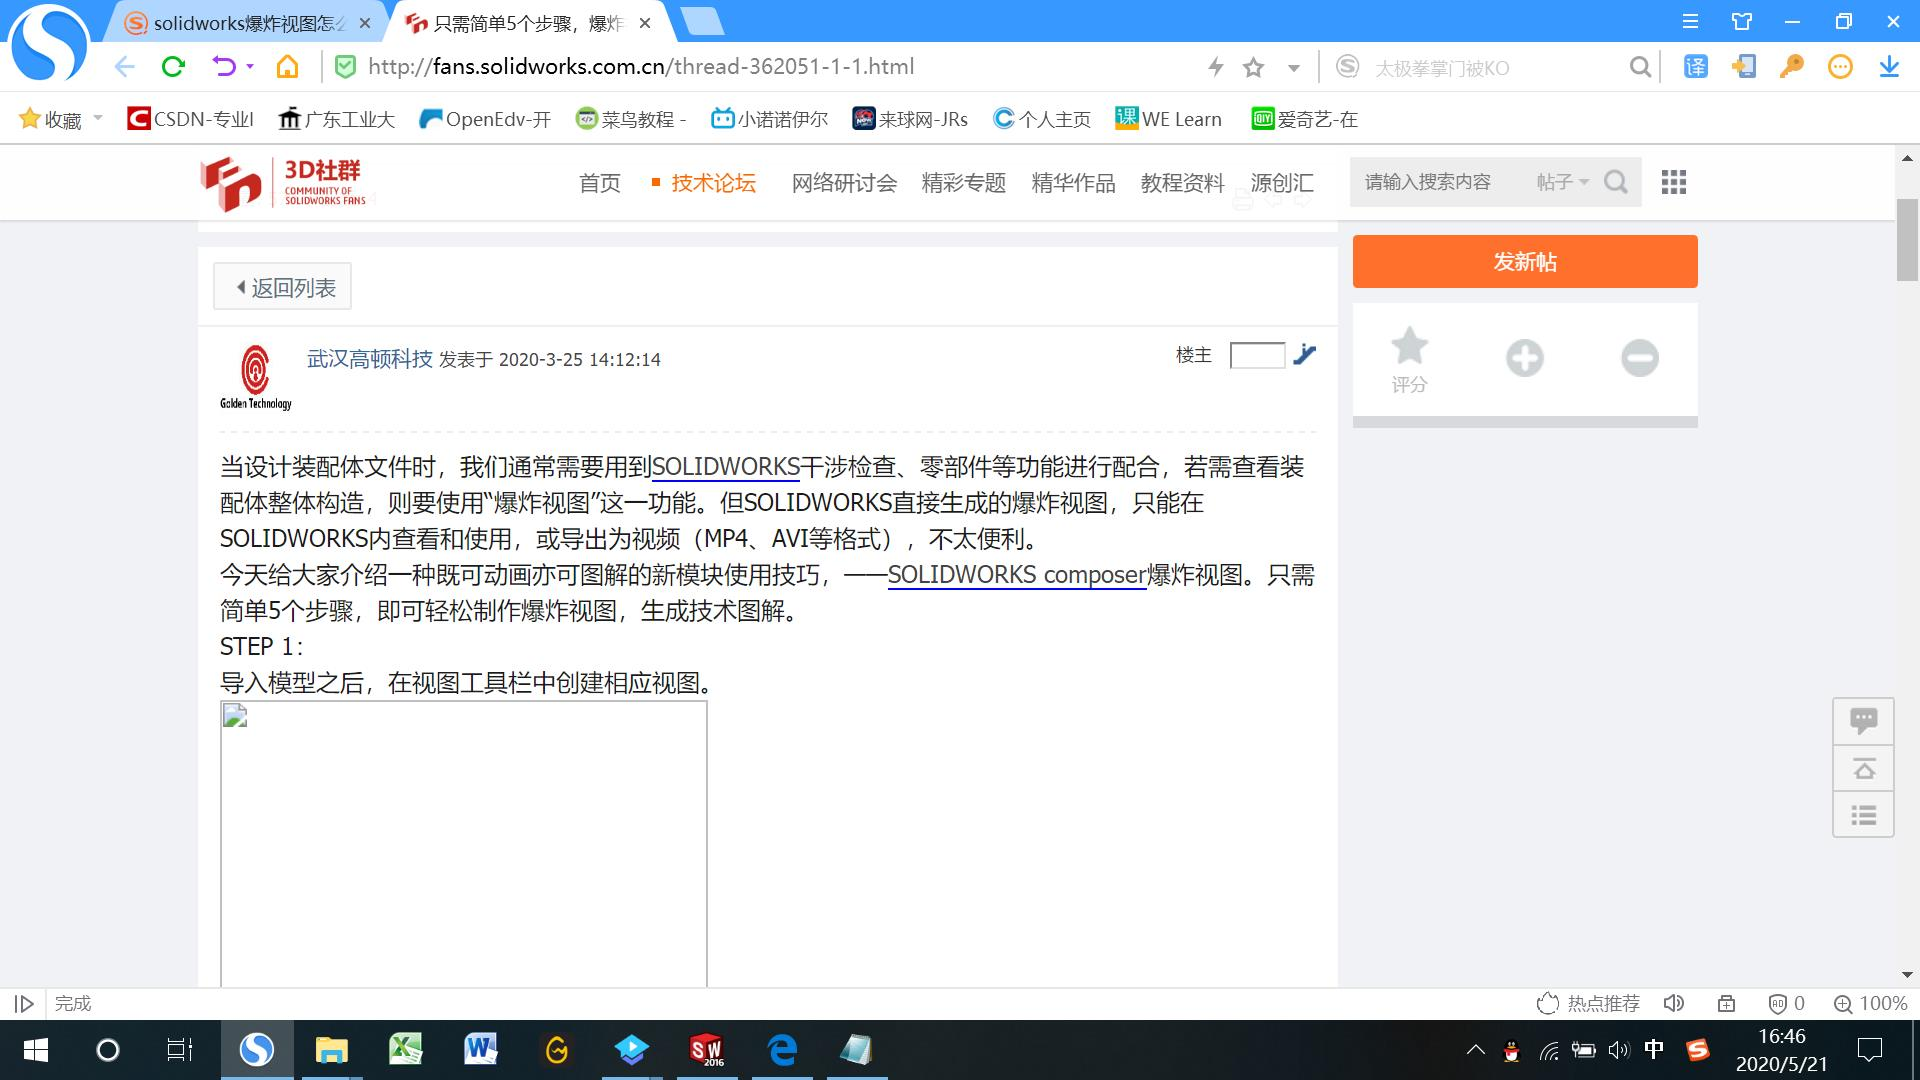
\includegraphics[width=12cm]{figure/1.jpg}
        \songti\zihao{5}\caption{脉冲发生模块程序流程图}
        \label{脉冲发生模块程序流程图}
    \end{figure}
    
  
    \subsubsection{检测计数模块}
    \songti\zihao{-4}{
    该模块功能在于,对到达指定位置的钢化玻璃进行计数,可以准确得知流水线上到位钢化玻璃的数量,便于后续统计。
    \begin{figure}[H]
        \centering
        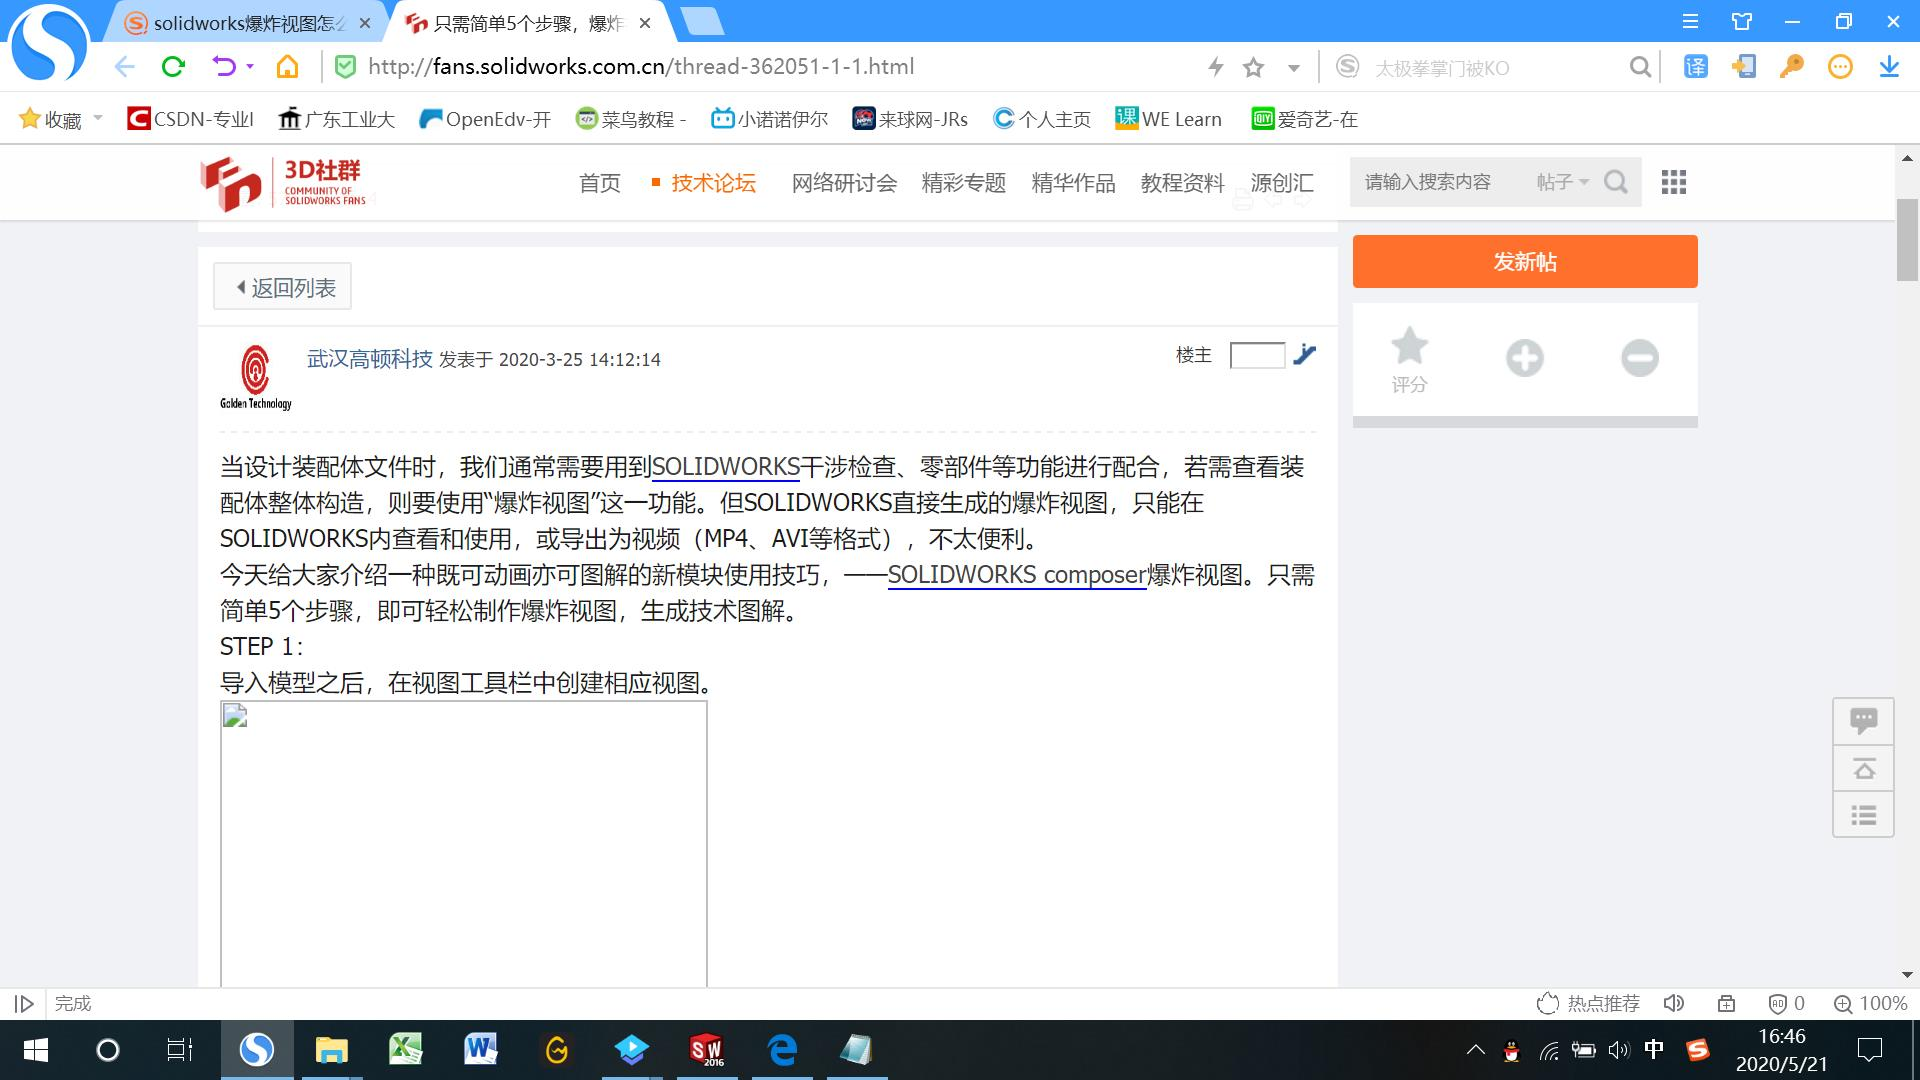
\includegraphics[width=10cm]{figure/1.jpg}
        \songti\zihao{5}{\caption{检测计数模块流程图}}
        \label{检测计数模块流程图}
    \end{figure}

    其功能实现流程如图\ref{检测计数模块流程图}示:当一块玻璃到位后,到位检测指示灯LED1变亮,CPLD芯片从CT\_1口得到一个高电平信号,计数寄存器object\_num加1;当钢化玻璃离开检测区域后,检测指示灯灭,等待下一块玻璃到位。\par
    
    }   
    
    \subsubsection{仿真模拟}
    